\subsection{Bottum-Up Mergesort}

Der Bottom-Up Mergesort Algorithmus besteht aus zwei Teilen: Einer Merge-Funktion und zwei verschachtelten schleifen, welche mit Hilfe von Merge ein Array sortieren. In dieser Implementierung wurde eine bitonische Variante von Merge verwendet, bei welcher zwei gegenläufig sortierte Hälften miteinander verschmolzen werden.


\begin{figure}[htbp] 
	\centering
	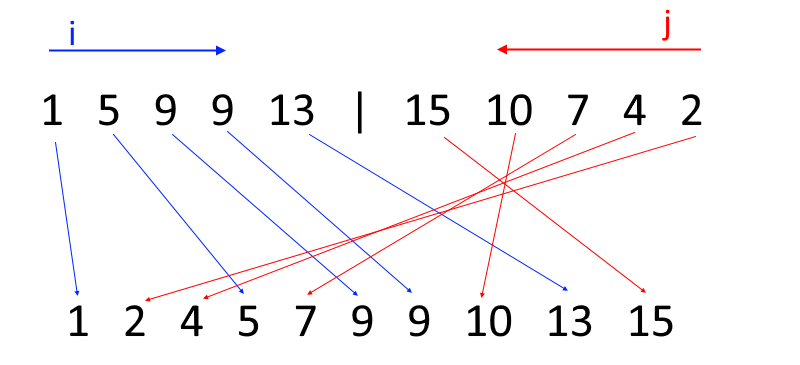
\includegraphics[width=0.5\textwidth]{./img/bionic-merge}
	\caption{Bitonische Variante von Mergesort.}
\end{figure}

\noindent
Bottom-Up Mergesort ist nicht rekursiv implementiert, sondern wir stattdessen mit zwei Schleifen realisiert. Für das Merge wird ein zweiten Array für Zwischenwerten benötigt. In einer effizienten Implementierung wird dieser Zwischenspeicher nur einmal erzeugt und für jeden Merge-Schritt wiederverwendet. Die Komplexität des Algorithmus beträgt $O(n*log(n))$.

\begin{PseudoCode}
	A := array with comparable elements;
	C := array as cache;
	for len = 1 to n do
		for lo = 0 to n - len do
			mid := len + lo - 1;
			hi := min(lo + 2 * len - 1, n - 1);
			merge(A, C, lo, mid, hi);
		end for	
	end for
\end{PseudoCode}

\noindent
\textbf{Beispiel 3.4.1 - Ausführung von Bottom-Up Mergesort}

\noindent
Der Algorithmus beginnt mit Teilarrays der Größe $len=1$.
\begin{equation*}
	\{4\},\;\{15\},\;\{9\},\;\{1\},\;\{10\},\;\{7\},\;\{9\},\;\{13\},\;\{2\},\;\{5\}
\end{equation*}
\newpage
\noindent
Anschließend werden die Elemente zu Arrays der Größe $2$ zusammengeführt.
\begin{gather*}
	\{4\},\;\{15\},\;\{9\},\;\{1\},\;\{10\},\;\{7\},\;\{9\},\;\{13\},\;\{2\},\;\{5\}\\
	\{4, 15\},\;\{1, 9\},\;\{7, 10\},\;\{9, 13\},\;\{2, 5\}
\end{gather*}
\noindent
Dieser Schritt wiederholt sich jetzt mit den Arrays der Größe $2$. Diese werden zu Arrays der Größe 4 verschmolzen. Ausnahme ist das letzte, da die Anzahl der Arrays ungerade ist.
\begin{gather*}
	\{4, 15\},\;\{1, 9\},\;\{7, 10\},\;\{9, 13\},\;\{2, 5\}\\
	\{1, 4, 9, 15\},\;\{7, 9, 10, 13\},\;\{2, 5\}
\end{gather*}
\noindent
Im nächsten Schritt werden die Arrays der Größe 4 miteinander verschmolzen, es verbleibt wieder das letzte Array der Größe 2.
\begin{gather*}
	\{1, 4, 9, 15\},\;\{7, 9, 10, 13\},\;\{2, 5\}\\
	\{1, 4, 7, 9, 9, 10, 13, 15\},\;\{2, 5\}
\end{gather*}
\noindent
Schließlich wird das verbleibende Array der Länge 2 mit dem Rest verschmolzen. Das Ergebnis ist ein aufsteigend sortiertes Array.
\begin{gather*}
	\{1, 4, 7, 9, 9, 10, 13, 15\},\;\{2, 5\}\\
	\{1, 2, 4, 5, 7, 9, 9, 10, 13, 15\}
\end{gather*}